\documentclass[runningheads]{llncs}

\usepackage[T1]{fontenc}
\usepackage[brazil]{babel}
\usepackage{graphicx}
\usepackage{amsmath}
\usepackage[colorlinks=true,linkcolor=black,citecolor=black,urlcolor=black]{hyperref}

% Parâmetros de comprimento que a própria classe llncs expõe para
% espaçamento de figura/legenda (distintos de overrides via
% \vspace/\textheight/baselinestretch, que o llncs.cls pede
% explicitamente para não usar e reseta após \begin{document} de
% qualquer forma).
\setlength{\abovecaptionskip}{4pt}
\setlength{\belowcaptionskip}{2pt}
\setlength{\floatsep}{6pt plus 2pt minus 2pt}
\setlength{\textfloatsep}{10pt plus 2pt minus 4pt}
\setlength{\intextsep}{6pt plus 2pt minus 2pt}

\begin{document}

\title{Fusão por Filtro de Kalman Estendido de Detecção Visual e Odometria sob Observação Esparsa: um Estudo de Caso em Gêmeo Digital Multi-Robô}

\titlerunning{Fusão EKF sob Observação Esparsa}

% Revisão double-blind: autor/instituição/e-mail/agradecimentos removidos.
% Restaurar somente na versão camera-ready pós-aceite.
\author{Anonymous Author(s)}

\authorrunning{Anonymous et al.}

\institute{Institution withheld for double-blind review}

\maketitle

\begin{abstract}
No gêmeo digital estudado aqui, sistemas multi-robô que combinam
odometria com detecção visual externa recorriam a um fallback
discreto: confiar na detecção quando disponível, na odometria caso
contrário. Essa abordagem descarta a incerteza de cada estimativa e
não oferece um comportamento bem definido durante lacunas de detecção.
Para resolver isso, substituímos o fallback por um Filtro de Kalman
Estendido (EKF) por robô, fundindo odometria e detecção visual
baseada em YOLO a partir de uma câmera fixa suspensa, validado em
duas etapas: primeiro consistência estatística em dados sintéticos
(NEES/NIS), depois avaliação em dados reais gravados, num gêmeo
digital ROS2/Gazebo com três robôs TurtleBot3.

O resultado depende de como o erro é medido. Nos instantes de
correção, o filtro reduz o erro de posição em $+23,7\%$ em relação à
odometria isolada sob deriva agressiva, o ganho que a literatura
tipicamente reporta. Mas, medido continuamente, a cada leitura de
odometria, o mesmo filtro é $12,7\%$ \emph{pior} que a odometria bruta,
sob a cobertura visual esparsa (0--28\%) que nossa câmera exibe na
prática. Mostramos que essa reversão de sinal é a consequência
esperada de operar abaixo de uma taxa crítica de observação, não uma
falha de projeto, e a conectamos mecanicamente a um teto de
covariância necessário para manter estável a associação por gating de
Mahalanobis. Reportar as duas métricas, e não apenas o ganho pontual
comumente citado, é necessário para caracterizar honestamente a fusão
por EKF sob observação esparsa; discutimos também por que filtros
alternativos (UKF, filtro de partículas, IMM) não resolvem essa
limitação, já que ela decorre da taxa de observação, não da escolha
do filtro.

\keywords{Filtro de Kalman Estendido \and Observações Intermitentes \and Localização Cooperativa \and Fusão Sensorial Assíncrona \and Localização Multi-Robô}
\end{abstract}

\section{Introdução}

Câmeras fixas suspensas observando múltiplos robôs móveis são
infraestrutura comum em automação de armazéns, coordenação de frotas
em ambientes internos e monitoramento de ambientes inteligentes, onde
instalar uma carga sensorial dedicada em cada robô é custosa ou
inviável. Sistemas multi-robô que combinam odometria embarcada com
essa detecção visual externa enfrentam uma escolha recorrente: como
combinar duas estimativas de posição ruidosas, que chegam em taxas
diferentes e nem sempre estão disponíveis no mesmo instante. Uma
solução comum e pragmática, usada no gêmeo digital estudado aqui antes
de nossa contribuição, é um \emph{fallback discreto}: confiar na
detecção quando associada com confiança, na odometria caso contrário.
Essa abordagem descarta informação: não há correção parcial a partir
de detecções de baixa confiança, nem propagação de incerteza, nem
comportamento bem definido durante trechos sem detecção.

A Filtragem de Kalman Estendida (EKF) é a resposta clássica a esse
problema, oferecendo predição e correção probabilística com
propagação explícita de incerteza. Suas propriedades de convergência,
no entanto, são classicamente estabelecidas sob observação
razoavelmente densa e regular~\cite{dissanayake2001slam}, uma
suposição que uma única câmera fixa suspensa, sujeita a campo de
visão finito e auto-oclusão durante manobras, não satisfaz em geral.
Este trabalho investiga se essa violação importa na prática.

Substituímos o fallback discreto por um EKF por robô, fundindo
odometria e detecção visual baseada em YOLO, avaliado de ponta a ponta
no mesmo gêmeo digital. Nossa contribuição é dupla. Primeiro,
validado em duas etapas, NEES/NIS sintético e depois dados reais
gravados, o filtro entrega um ganho de fusão real: $+23,7\%$ de
redução do erro de posição nos instantes de correção, sob deriva
agressiva. Segundo, o mesmo filtro, medido continuamente e não apenas
nos instantes de correção, é $12,7\%$ pior que a odometria bruta sob
a cobertura visual esparsa (0--28\%) que nossa câmera exibe na
prática. Explicamos essa reversão mecanicamente, conectando-a à
teoria já estabelecida sobre filtragem de Kalman sob observações
intermitentes~\cite{sinopoli2004intermittent,censi2009geometric}.
Argumentamos que reportar ambas as métricas é necessário para uma
caracterização honesta, e discutimos por que filtros alternativos não
resolvem a limitação subjacente.

\section{Trabalhos Relacionados}
\label{sec:related-work}

Durrant-Whyte e Bailey~\cite{bailey2006slam} formalizam o modelo
padrão de movimento/observação do EKF que nosso filtro segue
diretamente (odometria conduz a predição, detecções YOLO conduzem a
correção; notação adotada na Seção~\ref{sec:methodology}). Dissanayake
et al.~\cite{dissanayake2001slam} provam a convergência de covariância
do EKF-SLAM sob observação \emph{densa} de marcos, uma suposição que
nossa câmera com 0--28\% de cobertura viola por construção (central à
Seção~\ref{sec:discussion}). Sinopoli et
al.~\cite{sinopoli2004intermittent} estabelecem que, sob chegada de
observação de Bernoulli, a covariância diverge abaixo de uma taxa
crítica; nosso Cenário~3 (0\% de cobertura observada) é consistente
com o caso limite $p\to0$, de modo que a saturação observada é
teoricamente esperada, não um sintoma de má configuração. Censi~\cite{censi2009geometric}
observa que esse limiar crítico depende da métrica de resumo de
covariância usada; reportamos $\mathrm{trace}(P)$ como uma escolha de
escopo, não uma alegação de independência de métrica.

Arquiteturas de fusão que reportam um único número de ganho no
instante de correção são comuns na literatura de localização
multi-robô, mas nenhuma de que temos conhecimento também reporta um
regime de erro contínuo em que a fusão perde para a linha de base sem
fusão: o achado diferenciador deste trabalho. Nossa contribuição é o
relato conjunto do ganho no instante de correção e da degradação do
erro contínuo, fundamentado em
\cite{sinopoli2004intermittent,censi2009geometric} para explicar por
que esse trade-off é esperado, e não um bug de implementação. Também
não avaliamos contra um benchmark multi-robô público, já que esses
tipicamente assumem uma carga sensorial transportada por cada robô,
enquanto nossa configuração observa os robôs a partir de uma única
câmera externa e estática, mais próxima de um sensor fixo de ambiente
inteligente do que de SLAM cooperativo. Até onde sabemos, nenhum
conjunto de dados público combina esses elementos, o que motiva o
conjunto de dados gravado e disponibilizado com este trabalho
(Seção~\ref{sec:experimental-setup}). Esta cobertura reflete busca
direcionada, não uma revisão sistemática da literatura com protocolo
registrado; uma revisão formal continua em aberto.

\section{Método}
\label{sec:methodology}

Seguindo Durrant-Whyte e Bailey~\cite{bailey2006slam}, cada robô é
rastreado por um EKF independente com estado
$x_k=[p_x,p_y,\theta]^\top$. O modelo de movimento integra o
\emph{delta} entre leituras consecutivas de odometria sobre o estado
atual, não o valor absoluto, o que descartaria correções visuais
anteriores. O modelo de observação mapeia o estado para a posição 2D
reportada por um detector YOLO em uma câmera fixa suspensa
(Seção~\ref{sec:experimental-setup}).

\textbf{Predição e teto de covariância.} O ruído de processo é
$Q=\mathrm{diag}(0,5;\,0,5;\,0,25)$, escalado por $\Delta t/0,1$ para a
taxa real de odometria ($\approx$29\,Hz vs.\ os 0,1s assumidos na
calibração sintética); calibrado empiricamente (uma varredura de
$10^{-6}$ a $1,0$ mostrou ganho monotonicamente crescente até a
saturação em $Q\ge0,5$). Um teto rígido $\mathrm{clip}(P,-\infty,0,05)$
(elemento a elemento) é aplicado após cada predição: sem ele, $P$
crescia sem limite durante intervalos longos sem correção
($\mathrm{trace}(P)\approx85$ observado vs.\ $\approx0,5$ esperado),
quebrando a associação por gating de Mahalanobis ao alargar a região
de aceitação de um robô o suficiente para reivindicar a detecção de um
vizinho. Tanto $Q$ quanto esse teto foram calibrados exclusivamente
contra o ganho no instante de correção na
Tabela~\ref{tab:correction-error}; a degradação de erro contínuo
reportada adiante é, portanto, uma consequência observada dessa
escolha, não um trade-off conjuntamente otimizado. Essa é uma resposta
de engenharia à divergência que Sinopoli et
al.~\cite{sinopoli2004intermittent} caracterizam para sistemas
lineares abaixo de uma taxa crítica de observação; o resultado análogo
para o EKF é apenas local, condicional a ruído e erro inicial pequenos
o suficiente~\cite{kluge2010stochastic}, de modo que tratamos essa
conexão como motivação mecanicista, não como garantia formal para
nosso filtro não linear. O teto troca otimalidade estrita por
comportamento limitado e previsível sob observação esparsa.

\textbf{Associação de dados e correção.}
\label{sec:association}
Cada detecção é atribuída via vizinho mais próximo com gating de
Mahalanobis: $d^2=e^\top P_{xy}^{-1}e$ por par (robô, detecção),
aceito apenas se $d^2\le9,21$ (99\% de confiança, $\chi^2$, 2 graus de
liberdade). Isso herda uma limitação conhecida (Altendorfer e
Wirkert~\cite{altendorfer2016association}): uma covariância inflada
alarga a região de aceitação e pode enviesar a associação em direção a
trajetórias mais incertas, o mesmo modo de falha que motiva o teto de
covariância acima. Uma vez atribuída, o ruído de medição $R$ é
derivado linearmente da confiança de detecção do YOLO $c\in[0,1]$,
$\sigma=R_{\min}+(1-c)(R_{\max}-R_{\min})$, $R_{\min}=0,02$,
$R_{\max}=0,20$\,m.

\textbf{Calibração de câmera.} Os intrínsecos vêm de
\texttt{cv2.calibrateCamera} (método de Zhang). Uma
primeira tentativa com os quatro intrínsecos livres alcançou baixo
erro de reprojeção (0,162px), mas uma distância focal mal-condicionada
($f_x$ 33\% acima do valor teórico derivado do FOV): o caso degenerado
que o método de Zhang sofre quando o plano do tabuleiro permanece
fronto-paralelo ao sensor em todas as poses, inevitável com nossa
câmera fixa voltada para baixo. Corrigimos isso fixando
$f_x,f_y,c_x,c_y$ em seus valores nominais geométricos e calibrando
apenas a distorção da lente, o remédio padrão quando os intrínsecos
nominais já são conhecidos; a calibração corrigida reproduz a projeção
heurística já usada em produção com erro de até 0,001m, confirmando
que ambas são geometricamente equivalentes.

\textbf{Validação.} Seguindo os testes de consistência padrão para
filtros de Kalman, checamos primeiro NEES e NIS em simulação antes de confiar no filtro em dados reais: 30
sementes de Monte Carlo (2000 passos cada) fornecem NEES$=2,955$
(esperado $3,0$) e NIS$=1,982$ (esperado $2,0$), dentro de 1,5\%/0,9\%
de erro relativo, bem calibrado apesar de os limites formais de
$\chi^2$ a 95\% serem estreitos demais para passar nesse tamanho de
amostra. O filtro calibrado é então executado contra odometria e
detecções YOLO reais gravadas do gêmeo digital ao vivo, onde a
cobertura de observação é esparsa e irregular por construção, não por
escolha de projeto.

\textbf{Configuração experimental.}
\label{sec:experimental-setup}
Avaliamos nosso EKF em um gêmeo digital ROS2/Gazebo: três unidades
TurtleBot3 Waffle junto a uma câmera fixa suspensa em $(0,0,3)$\,m,
$90^\circ$ de inclinação para baixo, $60^\circ$ de campo de visão
horizontal, $640\times480$@10\,Hz. Cada robô também publica odometria
($\approx$29\,Hz) e uma leitura de LiDAR 2D não utilizada
(Seção~\ref{sec:future-work}). A detecção de robôs usa um modelo YOLO
treinado em 375 quadros anotados da mesma câmera,
$\mathrm{mAP@0.5}=0,995$; a confiança é carregada no campo $z$ de
outra forma não utilizado da mensagem de detecção, para consumo
direto pela etapa de correção do EKF.

\begin{figure}[t]
\centering
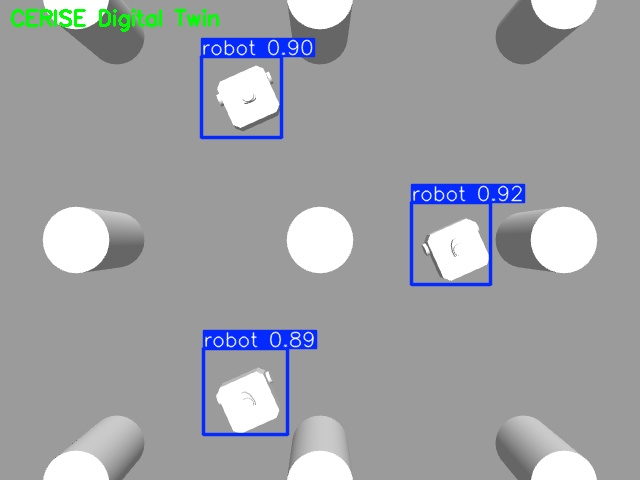
\includegraphics[width=0.55\textwidth]{figures/lafusion_pipeline_yolo_detection.jpg}
\caption{Vista aérea da câmera fixa sobre os três robôs TurtleBot3,
com as caixas delimitadoras e a confiança de detecção do modelo YOLO
sobrepostas em tempo real.}
\label{fig:yolo-detection}
\end{figure}

A Fig.~\ref{fig:yolo-detection} mostra a saída real desse pipeline de
detecção: os três robôs, vistos pela câmera fixa suspensa, com as
caixas delimitadoras e a confiança do YOLO sobrepostas.

Três cenários de $\sim$18\,s foram gravados como bags ROS2/MCAP: (a)
\textbf{Estacionário}: 152 detecções vs.\ 550 leituras de
odometria/robô, $\approx$28\% de cobertura, a mais alta dos três; (b)
\textbf{Movimento reto} ($v_x=0,1$\,m/s): 144 vs.\ 522 leituras,
$\approx$11\% de cobertura; (c) \textbf{Curva/oclusão} ($v_x=0,12$\,m/s,
$\omega_z=0,4$\,rad/s): 145 detecções registradas, mas \textbf{zero}
associadas com sucesso ao \texttt{robot1} durante toda a gravação,
produzindo o caso de cobertura 0\% central para a
Seção~\ref{sec:results}. A sincronização de timestamp foi verificada
via \texttt{rosbag2\_py} (nenhuma lacuna $>$500\,ms), descartando
dessincronização de relógio de sensor como fator de confusão.

Disponibilizamos um pacote de reprodutibilidade (arquivo de mundo,
URDF, calibração, hiperparâmetros do EKF, SHA do commit de código) e
documentamos uma dependência não óbvia:
\texttt{ros-humble-rosbag2-storage-mcap} não vem instalado por padrão
no ROS2 Humble.

\section{Resultados e Discussão}
\label{sec:results}

Reportamos duas métricas de erro distintas, deliberadamente mantidas
separadas: \emph{erro no instante de correção}, medido apenas quando
uma detecção YOLO é associada e fundida com sucesso (a mais comumente
reportada em trabalhos relacionados; Seção~\ref{sec:related-work}), e
\emph{erro contínuo}, medido a cada leitura de odometria
independentemente de correção. Essas duas métricas discordam em
sinal, e ambas são necessárias para caracterizar honestamente o
comportamento do filtro sob observação esparsa.

\textbf{Erro no instante de correção.}
A validação NEES/NIS sintética (Seção~\ref{sec:methodology}) confirma
que o filtro está bem calibrado antes de qualquer avaliação com dados
reais (Fig.~\ref{fig:nees-nis}, NEES$\to 3,0$, NIS$\to 2,0$).

\begin{figure}[t]
\centering
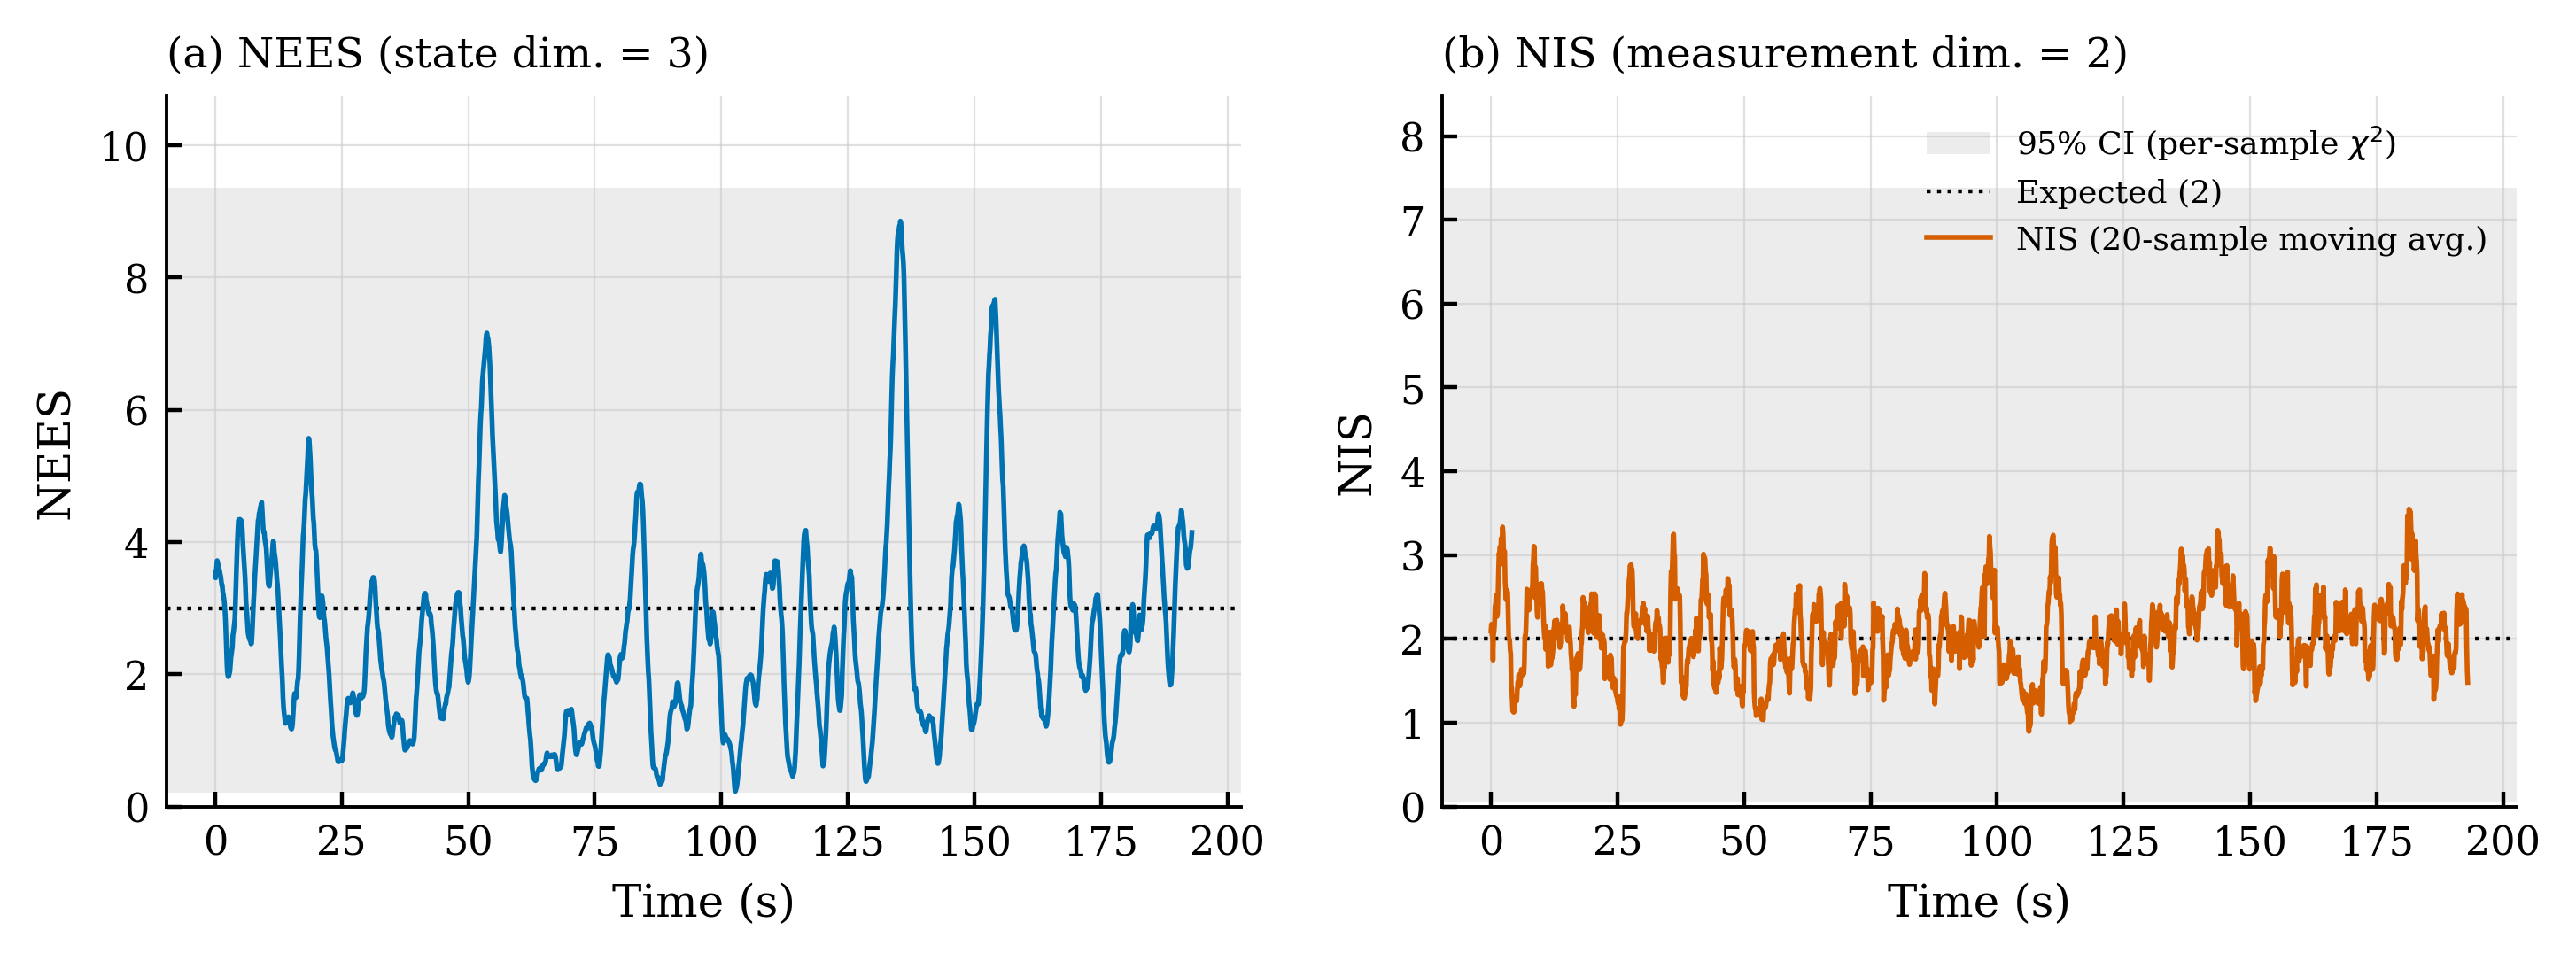
\includegraphics[width=0.95\textwidth]{figures/lafusion_nees_nis.png}
\caption{Consistência de NEES e NIS ao longo da validação sintética de
Monte Carlo (30 sementes, 2000 passos cada). Ambas as estatísticas
acompanham seus valores teóricos esperados, indicando um filtro bem
calibrado.}
\label{fig:nees-nis}
\end{figure}

A Tabela~\ref{tab:correction-error} reporta o erro de posição sob três
regimes de deriva de odometria injetada, agregados nos três cenários
gravados ($n=1323$). Sob deriva agressiva, o regime em que a odometria
bruta já acumulou erro substancial antes que uma correção visual se
torne disponível, o EKF reduz o erro médio de posição em $+23,7\%$ em
relação à odometria isolada (teste de postos sinalizados de Wilcoxon,
$p<0,001$; as amostras dentro de um cenário são temporalmente
autocorrelacionadas, de modo que esse $n$ superestima o número de
tentativas independentes, e o $p$-valor deve ser lido como otimista,
limitação agravada pelo fato de cada cenário durar apenas
$\sim$18\,s). Sob deriva leve, o ganho é negativo ($-5,3\%$): o erro
de detecção visual ($\approx$3--6\,cm) ainda não é menor que o erro de
odometria, já pequeno, de modo que a fusão não oferece benefício,
comportamento esperado para um filtro corretamente calibrado, não uma
falha.

\begin{table}
\caption{Erro de posição no instante de correção (m), agregado nos 3
cenários ($n=1323$). Cada célula reporta EKF~/~apenas odometria; as
colunas $\Delta$ dão a redução relativa do EKF.}\label{tab:correction-error}
\footnotesize
\begin{tabular}{|l|c|c|c|c|}
\hline
\textbf{Deriva} & \textbf{Média EKF/Odom} & \textbf{Média $\Delta$} & \textbf{RMSE EKF/Odom} & \textbf{RMSE $\Delta$} \\
\hline
Nenhuma (odom=GT) & 0,036 / 0,000 & N/D & 0,052 / 0,000 & N/D \\
\hline
Leve & 0,053 / 0,050 & $-5,3\%$ & 0,068 / 0,066 & $-2,1\%$ \\
\hline
Agressiva & 0,128 / 0,168 & $\mathbf{+23,7\%}$ & 0,163 / 0,195 & $\mathbf{+16,7\%}$ \\
\hline
\end{tabular}
\end{table}

\begin{figure}[t]
\centering
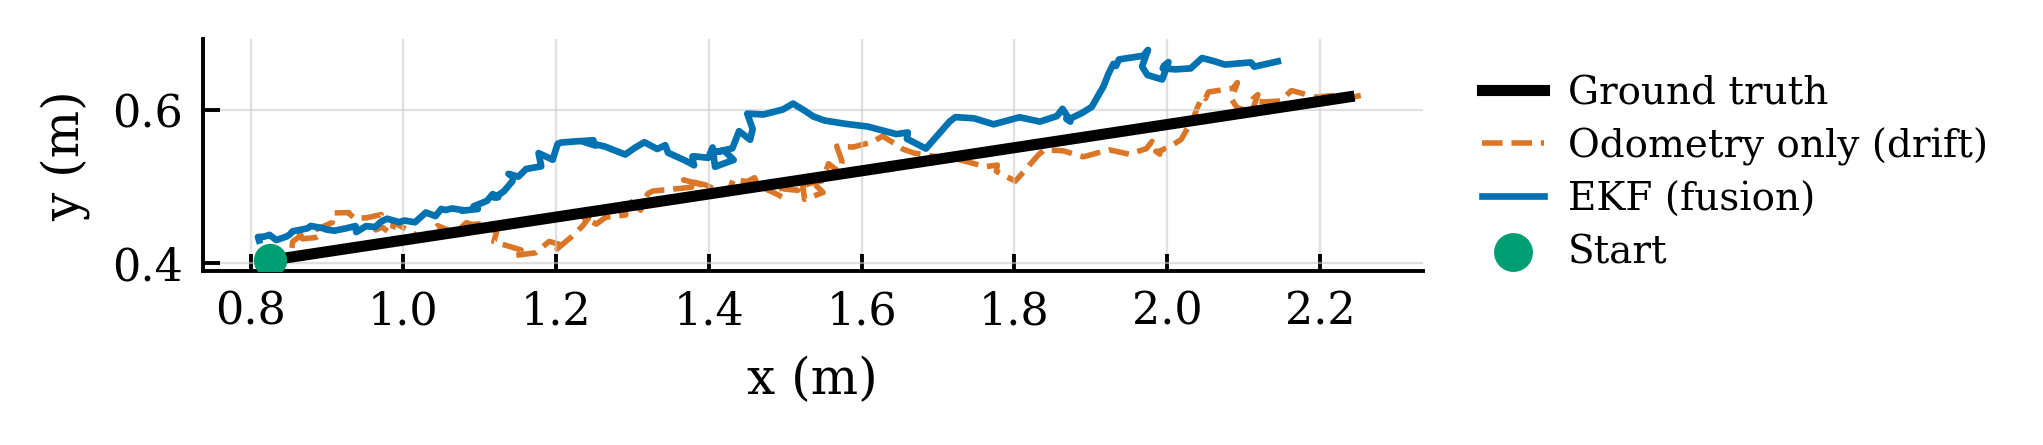
\includegraphics[width=0.75\textwidth]{figures/lafusion_trajectory.png}
\caption{Trajetória estimada sob deriva agressiva, Cenário 2
(movimento reto). O EKF (azul) acompanha a ground truth (preto) mais
de perto que a odometria bruta com deriva (laranja, tracejado).}
\label{fig:trajectory}
\end{figure}

A Fig.~\ref{fig:trajectory} mostra isso qualitativamente: a odometria
bruta visivelmente se afasta do caminho reto de ground truth, enquanto
a estimativa do EKF o acompanha mais de perto.

\textbf{Erro contínuo: o achado central.}
Quando o erro é medido a \emph{cada} leitura de odometria, o resultado
se inverte. A Tabela~\ref{tab:continuous-error} reporta o erro em
tempo contínuo sob deriva agressiva, usando as mesmas gravações.
Agregado em todas as leituras ($n=1607$), o EKF é $12,7\%$ \emph{pior}
que a odometria bruta pelo erro médio e $13,4\%$ pior pelo RMSE (teste
de postos sinalizados de Wilcoxon, $p<0,001$), o sinal oposto ao
resultado no instante de correção, com o RMSE confirmando a mesma
reversão, não um artefato da métrica de erro médio.

\begin{table}
\caption{Erro de posição contínuo (m), a cada leitura de odometria,
deriva agressiva. Cada célula reporta EKF~/~apenas odometria; a
mudança de RMSE confirma a mesma reversão do erro médio.}\label{tab:continuous-error}
\footnotesize
\begin{tabular}{|l|c|c|c|c|c|}
\hline
\textbf{Cenário} & \textbf{Cob.} & \textbf{Média EKF/Odom} & \textbf{Média $\Delta$} & \textbf{RMSE EKF/Odom} & \textbf{RMSE $\Delta$} \\
\hline
Estacionário & 27,6\% & 0,212 / 0,177 & $-19,3\%$ & 0,246 / 0,205 & $-19,8\%$ \\
\hline
Reto & 11,3\% & 0,212 / 0,178 & $-18,8\%$ & 0,245 / 0,206 & $-19,2\%$ \\
\hline
Curva/ocl. & 0,0\% & 0,178 / 0,178 & $-0,0\%$ & 0,205 / 0,205 & $-0,0\%$ \\
\hline
\textbf{Agregado} & --- & \textbf{0,200 / 0,178} & $\mathbf{-12,7\%}$ & \textbf{0,233 / 0,205} & $\mathbf{-13,4\%}$ \\
\hline
\end{tabular}
\end{table}

O erro acima segue a convenção de Erro de Trajetória Absoluto (ATE) de
Sturm et al.~\cite{sturm2012tum}: erro de posição por amostra contra a
ground truth, sem alinhamento rígido, apropriado aqui porque
estimativa, odometria e ground truth já compartilham um referencial de
mundo comum via a câmera fixa (diferentemente de SLAM, onde a
trajetória tem um gauge livre). O ATE isoladamente não consegue
distinguir se a degradação vem do erro acumulando ao longo do tempo ou
de cada passo já derivando mais. Por isso também reportamos o Erro de
Pose Relativo (RPE)~\cite{sturm2012tum}: o erro do delta de posição
entre leituras consecutivas, isolando o desvio local do erro global
acumulado que o ATE captura. Agregado nos cenários, o RPE é $4,2\%$
pior pelo erro médio e $4,8\%$ pior pelo RMSE, o mesmo sinal do ATE
mas substancialmente menor, indicando que a reversão é impulsionada
majoritariamente pelo erro acumulando ao longo do tempo sob correção
esparsa, não pelo desvio passo a passo.

Duas observações explicam essa reversão. Primeiro, a degradação
escala inversamente com a cobertura do YOLO: o Cenário 3 (0\% de
cobertura) mostra uma mudança de exatamente $0,0\%$, porque, com zero
correções, a etapa de predição do EKF degenera para pura integração de
delta de odometria, idêntica matematicamente à linha de base sem
fusão. Os Cenários 1 e 2 (27,6\% e 11,3\% de cobertura) mostram
degradação semelhante de $\sim$19\% apesar de níveis de cobertura
diferentes, sugerindo que o efeito satura rapidamente assim que as
correções ficam esparsas o bastante para o teto de covariância
(Seção~\ref{sec:methodology}) entrar em ação.

\begin{figure}[t]
\centering

\includegraphics[width=0.9\textwidth]{figures/lafusion_covariance_trace.png}
\caption{Saturação da covariância de posição ao longo do tempo
(gráficos em degraus), nos três cenários, sob duas métricas (topo:
$\mathrm{trace}(P_{xy})$; base: $\lambda_{max}(P_{xy})$, o maior
autovalor), seguindo a observação de
Censi~\cite{censi2009geometric} de que o limiar crítico de observação
depende da métrica de erro escolhida. Traços verticais na base de cada
painel marcam correções YOLO bem-sucedidas. Linhas tracejadas marcam o
teto de cada métrica sob o mesmo clip elemento a elemento
(Seção~\ref{sec:methodology}): $2\times\mathrm{COV\_CAP}=0,1$ para o
traço e $\mathrm{COV\_CAP}=0,05$ para o maior autovalor isoladamente.
Ambas as métricas concordam qualitativamente: a cobertura diminui da
esquerda para a direita (27,6\% $\to$ 11,3\% $\to$ 0\%), e a
covariância satura em seu teto por trechos correspondentemente mais
longos, atingindo saturação permanente no caso de cobertura zero.}
\label{fig:covariance-trace}
\end{figure}

Segundo, e explicando mecanicamente o primeiro, a
Fig.~\ref{fig:covariance-trace} mostra o porquê: $\mathrm{trace}(P)$
satura no teto de covariância quase imediatamente após qualquer
intervalo sem correção, e só cai quando uma correção ocorre. No
Cenário 3, o traço satura já no primeiro passo observado e nunca mais
cai. Esse é precisamente o regime de divergência previsto por Sinopoli
et al.~\cite{sinopoli2004intermittent} para taxas de chegada de
observação abaixo de um limiar crítico: o teto de covariância impede
crescimento sem limite (e as falhas de associação que causaria) ao
limitar a \emph{própria estimativa de incerteza} do filtro, não
tornando sua estimativa de estado mais precisa durante o intervalo sem
correção: o filtro permanece superconfiante em sua predição baseada
apenas em odometria, em relação a quão incerta essa predição realmente
é.

\textbf{Discussão.}
\label{sec:discussion}
A leitura natural da Tabela~\ref{tab:continuous-error} é desfavorável:
nosso EKF, avaliado continuamente, perde para a odometria que deveria
melhorar. Argumentamos que isso é esperado, não um projeto falho. A
prova de convergência de Dissanayake et
al.~\cite{dissanayake2001slam} assume observação densa; nossa câmera
viola isso por construção (0--28\% de cobertura), e Sinopoli et
al.~\cite{sinopoli2004intermittent} preveem exatamente essa divergência
de covariância sem um teto, e a superconfiança resultante com um teto
presente. A mudança de $0,0\%$ do Cenário~3 é uma confirmação limpa:
com zero correções, a etapa de predição é comprovadamente idêntica à
integração de delta de odometria. Seguimos
Censi~\cite{censi2009geometric} ao reportar $\mathrm{trace}(P)$ como
uma escolha de escopo, não uma alegação de divergência independente de
métrica.

Nenhuma alternativa padrão resolve o caso de cobertura zero: um filtro
de partículas degenera para pura propagação de processo, sem
verossimilhança para reponderar; um filtro IMM ainda exige alguma
observação para ponderar modos concorrentes; e um UKF visa a não
linearidade do modelo de observação, não a \emph{taxa} de observação,
distinção apoiada pelo fato de que uma divergência análoga em taxa
crítica já foi demonstrada para o UKF sob observações
intermitentes~\cite{li2012ukf}. Tratamos a baixa cobertura como a
causa raiz, consistente com a literatura de posicionamento de
sensores: limites de estimação sob uma dada topologia de sensor se
mantêm independentemente do filtro usado. O teto de covariância é,
portanto, uma aproximação de engenharia para manter uma estimativa de
estado limitada e previsível durante lacunas de observação, trocando
otimalidade por estabilidade de associação, e herda uma limitação de
gating conhecida (Altendorfer e
Wirkert~\cite{altendorfer2016association}): uma covariância saturada
alarga a região de aceitação precisamente quando a incerteza real é
pior caracterizada por um valor fixo, embora não tenhamos observado
associação cruzada incorreta entre robôs em nossos três cenários.

Testamos esse trade-off diretamente, em vez de apenas argumentá-lo. Um
fator de esquecimento (Adaptive Fading Kalman Filter), a alternativa
tecnicamente correta por preservar a estrutura semidefinida positiva
de $P$, foi implementado e avaliado sob o mesmo protocolo. Sem teto, o
ganho caiu de $+23,7\%$/$+16,7\%$ (clip) para $-18,5\%$/$-112,5\%$. Um
teto mais generoso recuperou um ganho positivo de erro médio na
configuração mais restritiva testada ($0,1$: $+9,1\%$ de média, mas
$-38,8\%$ de RMSE, indicando outliers grandes ocasionais), degradando
novamente conforme o teto se alarga ($0,2$: $-3,9\%$; $0,3$:
$-19,3\%$/$-111,3\%$). Nenhuma configuração igualou o clip nas duas
métricas simultaneamente, e as duas métricas discordaram em sinal na
única configuração em que o erro médio melhorou. Esse comportamento
não monotônico é, por si só, evidência contra o fator de esquecimento
como substituto direto: seu comportamento prático depende
sensivelmente de um hiperparâmetro adicional sem um padrão
principiado, e um teto mais frouxo ainda permite que $P$ cresça o
suficiente para a associação com gating de Mahalanobis aceitar a
detecção de um robô vizinho, o mesmo modo de falha que o clip existe
para evitar. Reportamos isso como evidência empírica, não apenas
justificativa teórica, para a escolha do clip.

\section{Trabalhos Futuros e Conclusão}

\textbf{Trabalhos futuros.}
\label{sec:future-work}
Direções concretas incluem: (a) \textbf{ruído de processo adaptativo}:
escalar $Q$ pelo tempo desde a última correção em vez de um teto fixo,
mais principiado mas, como nosso teste do fator de esquecimento
mostra, não uma melhora garantida sem ajuste adicional; (b)
\textbf{LiDAR como terceira fonte de fusão}: cada robô já publica
leituras 2D não utilizadas; correções mútuas via LiDAR entre robôs
poderiam mirar diretamente o regime de cobertura zero; (c)
\textbf{incerteza de projeção formal}: propagar o Jacobiano completo
de projeção para $R$; (d) \textbf{localização relativa distribuída}:
um canal de filtragem sem câmera na mesma plataforma poderia fornecer
um segundo canal de correção durante lacunas de cobertura visual.

\textbf{Conclusão.}
Substituímos um fallback discreto visual/odometria por um Filtro de
Kalman Estendido validado em duas etapas, avaliado em dados reais
gravados de três robôs TurtleBot3. O filtro entrega um ganho genuíno
nos instantes de correção ($+23,7\%$), mas é mensuravelmente pior que
a odometria bruta quando avaliado continuamente ($-12,7\%$) sob
0--28\% de cobertura visual, incluindo um cenário de cobertura zero
que colapsa, exatamente como esperado, para a linha de base sem fusão.
Em vez de reportar apenas a métrica favorável, caracterizamos ambas e
fundamentamos a reversão na teoria estabelecida sobre filtragem de
Kalman sob observação intermitente. A fusão por EKF continua sendo a
ferramenta certa para este problema, mas sua correção sob observação
esparsa precisa ser medida e reportada explicitamente, e a própria
taxa de observação, não a escolha do filtro, é a restrição vinculante
que trabalhos futuros devem mirar.

\begin{thebibliography}{8}
\setlength{\itemsep}{0pt}
\setlength{\parskip}{2pt}

\bibitem{kluge2010stochastic}
Kluge, S., Reif, K., Brokate, M.: Stochastic stability of the extended
Kalman filter with intermittent observations. IEEE Transactions on
Automatic Control \textbf{55}(2), 514--518 (2010)

\bibitem{li2012ukf}
Li, L., Xia, Y.: Stochastic stability of the unscented Kalman filter
with intermittent observations. Automatica \textbf{48}(5), 978--981
(2012)

\bibitem{bailey2006slam}
Durrant-Whyte, H., Bailey, T.: Simultaneous localization and mapping
(SLAM): Part I. IEEE Robotics \& Automation Magazine \textbf{13}(2),
99--110 (2006)

\bibitem{dissanayake2001slam}
Dissanayake, M.W.M.G., Newman, P., Clark, S., Durrant-Whyte, H.F.,
Csorba, M.: A solution to the simultaneous localization and map building
(SLAM) problem. IEEE Transactions on Robotics and Automation
\textbf{17}(3), 229--241 (2001)

\bibitem{sinopoli2004intermittent}
Sinopoli, B., Schenato, L., Franceschetti, M., Poolla, K., Jordan, M.I.,
Sastry, S.S.: Kalman filtering with intermittent observations. IEEE
Transactions on Automatic Control \textbf{49}(9), 1453--1464 (2004)

\bibitem{censi2009geometric}
Censi, A.: Geometric remarks on Kalman filtering with intermittent
observations. arXiv:0906.1637 (2009)

\bibitem{altendorfer2016association}
Altendorfer, R., Wirkert, S.J.: Why the association log-likelihood
distance should be used for measurement-to-track association. In: 2016
IEEE Intelligent Vehicles Symposium (IV). pp. 258--265 (2016)

\bibitem{sturm2012tum}
Sturm, J., Engelhard, N., Endres, F., Burgard, W., Cremers, D.: A
benchmark for the evaluation of RGB-D SLAM systems. In: 2012 IEEE/RSJ
International Conference on Intelligent Robots and Systems (IROS),
pp. 573--580 (2012)

\end{thebibliography}
\end{document}
